\documentclass[12pt,a4paper]{article}

% ── Packages ──────────────────────────────────────────────────────
\usepackage[T1]{fontenc}
\usepackage[utf8]{inputenc}
\usepackage[margin=2.5cm]{geometry}
\usepackage{amsmath,amssymb}
\usepackage{graphicx}
\usepackage{booktabs}
\usepackage{caption}
\usepackage{subcaption}
\usepackage{hyperref}
\usepackage{xcolor}
\usepackage{parskip}
\usepackage{float}
\usepackage{fancyhdr}
\setlength{\headheight}{14.5pt}
\usepackage{titlesec}
\usepackage{array}
\usepackage{multirow}
\usepackage{tikz}
\usetikzlibrary{arrows.meta, decorations.pathreplacing, shapes.geometric}
\definecolor{colEz}{RGB}{31,119,180}
\definecolor{colHx}{RGB}{214,39,40}
\definecolor{colHy}{RGB}{44,160,44}

% ── Header/footer ─────────────────────────────────────────────────
\pagestyle{fancy}
\fancyhf{}
\rhead{GP-GPU — FDTD 2D Parallelization}
\lhead{M2 — 2025/2026}
\cfoot{\thepage}

% ── Title ─────────────────────────────────────────────────────────
\title{
    \vspace{-1cm}
    \Large\textbf{Parallelization of the 2D Finite-Difference Time-Domain Method}\\[0.4em]
    \large Using OpenMP and CUDA\\[1em]
    \normalsize GP-GPU Project — M2
}
\author{Lucas Royer}
\date{February 2026}

% ── Equation shortcuts ────────────────────────────────────────────
\newcommand{\eps}{\varepsilon_0}
\newcommand{\muu}{\mu_0}

% ─────────────────────────────────────────────────────────────────
\begin{document}
\maketitle
\tableofcontents
\newpage

% =================================================================
\section*{Abstract}
\addcontentsline{toc}{section}{Abstract}
% =================================================================

The objective of this project is to parallelize the two-dimensional
Finite-Difference Time-Domain (FDTD) method (a standard algorithm
in computational electromagnetics) using two complementary
parallel programming models: OpenMP for multi-core CPU parallelism,
and CUDA for GPU acceleration.

The FDTD algorithm updates three electromagnetic field arrays
($E_z$, $H_x$, $H_y$) on a 2D Yee grid at every time step.
Its update equations are parallel: each cell depends
only on its immediate neighbors and not on other cells being updated
in the same pass.
Three implementations were developed and share a common interface:
a sequential baseline (\texttt{SequentialFDTD}), a multi-threaded
CPU version (\texttt{OpenMPFDTD}) using \texttt{\#pragma omp parallel for},
and a GPU version (\texttt{CudaFDTD}) that maps one CUDA thread
per grid cell.
Both Dirichlet (PEC cavity) and Perfectly Matched Layer (PML)
absorbing boundary conditions were implemented.

On a 200$\times$200 grid with 1000 time steps,
CUDA achieves a speedup of \textbf{3.85$\times$} over the sequential
reference, reaching 35.1~GFLOP/s and utilizing 96.6\% of the GPU's
theoretical memory bandwidth.
OpenMP provides no speedup at this grid size due to synchronization
overhead exceeding the computation gain, but scales beneficially on
larger grids (512$\times$512 and above).
Strong scaling experiments confirm that the GPU speedup grows from
1.94$\times$ at 128$\times$128 to \textbf{9.85$\times$} at
1024$\times$1024.
A Roofline analysis confirms the algorithm is memory-bound
($AI = 0.134$~FLOP/byte), explaining why GPU bandwidth
(272~GB/s) is the primary performance lever.

% =================================================================
\section{Design Methodology}
% =================================================================

\subsection{Overview of the FDTD Algorithm}

The Finite-Difference Time-Domain method numerically solves Maxwell's equations in the time domain by discretizing both space and time
on a staggered \emph{Yee grid}.
For the 2D transverse-electric (TE) polarization considered here,
three field components are evolved:
$E_z$, $H_x$, and $H_y$.
The update equations at each time step $n$ are:

\begin{align}
H_x^{n+1/2}(i,j) &= H_x^{n-1/2}(i,j)
    - \frac{\Delta t}{\mu_0\,\Delta y}
      \bigl[E_z^n(i,j+1) - E_z^n(i,j)\bigr]
\label{eq:hx}\\[4pt]
H_y^{n+1/2}(i,j) &= H_y^{n-1/2}(i,j)
    + \frac{\Delta t}{\mu_0\,\Delta x}
      \bigl[E_z^n(i+1,j) - E_z^n(i,j)\bigr]
\label{eq:hy}\\[4pt]
E_z^{n+1}(i,j)   &= E_z^n(i,j)
    + \frac{\Delta t}{\varepsilon_0}
      \left[
        \frac{H_y^{n+1/2}(i,j)-H_y^{n+1/2}(i-1,j)}{\Delta x}
        - \frac{H_x^{n+1/2}(i,j)-H_x^{n+1/2}(i,j-1)}{\Delta y}
      \right]
\label{eq:ez}
\end{align}

The time step satisfies the Courant–Friedrichs–Lewy stability condition:
\begin{equation}
    \Delta t = \frac{0.99}{\displaystyle c_0\sqrt{\frac{1}{\Delta x^2}+\frac{1}{\Delta y^2}}}
    \approx \frac{0.99\,\Delta x}{c_0\sqrt{2}}
\end{equation}
with $\Delta x = \Delta y = 1\,\text{mm}$, giving
$\Delta t \approx 2.36\,\text{ps}$.

The leapfrog time integration alternates half-steps for $\mathbf{H}$
and full steps for $E_z$ as illustrated in Figure~\ref{fig:yee}.
A point source injects energy at the center of the domain.

\begin{figure}[H]
  \centering
  \resizebox{\textwidth}{!}{% fig_yee_grid.tex — Grille de Yee 2D avec espacements optimisés
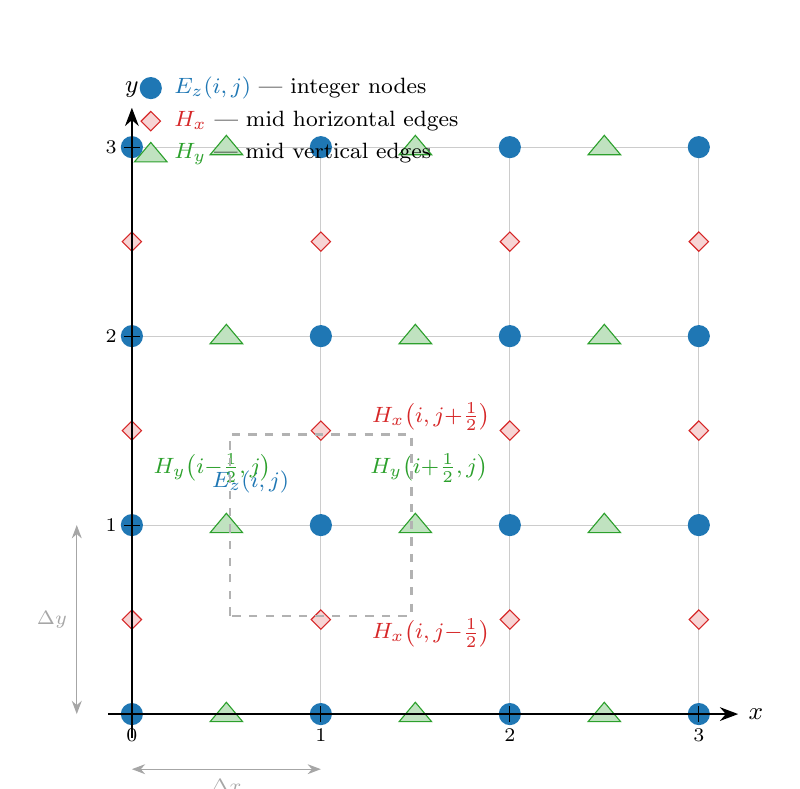
\begin{tikzpicture}[>=Stealth, font=\small]

\def\dx{2.4}
\def\dy{2.4}
\def\Nx{3}
\def\Ny{3}

% Grille
\foreach \i in {0,...,\Nx} {
    \draw[gray!40, thin] (\i*\dx, 0) -- (\i*\dx, \Ny*\dy);
}
\foreach \j in {0,...,\Ny} {
    \draw[gray!40, thin] (0, \j*\dy) -- (\Nx*\dx, \j*\dy);
}

% Ez aux nœuds entiers (i,j) — cercles bleus (taille réduite)
\foreach \i in {0,...,\Nx} {
    \foreach \j in {0,...,\Ny} {
        \fill[colEz] (\i*\dx, \j*\dy) circle (4pt);
    }
}

% Hx au milieu des arêtes horizontales — carrés rouges (taille réduite)
\foreach \i in {0,...,\Nx} {
    \foreach \j in {0,...,2} {
        \node[draw=colHx, fill=colHx!20, regular polygon,
              regular polygon sides=4, rotate=45,
              minimum size=7pt, inner sep=0pt]
            at (\i*\dx, \j*\dy + 0.5*\dy) {};
    }
}

% Hy au milieu des arêtes verticales — triangles verts (taille réduite)
\foreach \i in {0,...,2} {
    \foreach \j in {0,...,\Ny} {
        \node[draw=colHy, fill=colHy!30,
              isosceles triangle, isosceles triangle apex angle=80,
              rotate=90, minimum size=7pt, inner sep=0pt]
            at (\i*\dx + 0.5*\dx, \j*\dy) {};
    }
}

% Étiquettes cellule centrale (i=1, j=1) avec ancrages précis
\def\ci{1}
\def\cj{1}

% Étiquette Ez : placée au-dessus à gauche du cercle
\node[above left=8pt, colEz, font=\footnotesize\bfseries]
    at (\ci*\dx, \cj*\dy) {$E_z(i,j)$};

% Hx supérieur : à droite avec décalage vertical supplémentaire
\node[anchor=west, xshift=15pt, yshift=5pt, colHx, font=\footnotesize\bfseries]
    at (\ci*\dx, \cj*\dy + 0.5*\dy)
    {$H_x\!\left(i,j{+}\frac{1}{2}\right)$};

% Hx inférieur : à droite avec décalage vertical négatif
\node[anchor=west, xshift=15pt, yshift=-5pt, colHx, font=\footnotesize\bfseries]
    at (\ci*\dx, \cj*\dy - 0.5*\dy)
    {$H_x\!\left(i,j{-}\frac{1}{2}\right)$};

% Hy droite : au-dessus avec décalage horizontal
\node[anchor=south, yshift=12pt, xshift=5pt, colHy, font=\footnotesize\bfseries]
    at (\ci*\dx + 0.5*\dx, \cj*\dy)
    {$H_y\!\left(i{+}\frac{1}{2},j\right)$};

% Hy gauche : au-dessus avec décalage horizontal négatif
\node[anchor=south, yshift=12pt, xshift=-5pt, colHy, font=\footnotesize\bfseries]
    at (\ci*\dx - 0.5*\dx, \cj*\dy)
    {$H_y\!\left(i{-}\frac{1}{2},j\right)$};

% Rectangle cellule centrale
\draw[black!30, thick, dashed]
    (\ci*\dx-0.5*\dx+0.05, \cj*\dy-0.5*\dy+0.05)
    rectangle
    (\ci*\dx+0.5*\dx-0.05, \cj*\dy+0.5*\dy-0.05);

% Axes (inchangés)
\draw[->, thick] (-0.3, 0) -- (\Nx*\dx+0.5, 0) node[right] {$x$};
\draw[->, thick] (0, -0.3) -- (0, \Ny*\dy+0.5)  node[above] {$y$};
\foreach \i in {0,...,\Nx} {
    \draw[thin] (\i*\dx,-0.1)--(\i*\dx,0.1);
    \node[below=2pt,font=\scriptsize] at (\i*\dx,0) {$\i$};
}
\foreach \j in {1,...,\Ny} {
    \draw[thin] (-0.1,\j*\dy)--(0.1,\j*\dy);
    \node[left=2pt,font=\scriptsize] at (0,\j*\dy) {$\j$};
}
\draw[<->,thin,gray!70] (0,-0.7)--(\dx,-0.7)
    node[midway,below,font=\scriptsize] {$\Delta x$};
\draw[<->,thin,gray!70] (-0.7,0)--(-0.7,\dy)
    node[midway,left,font=\scriptsize]  {$\Delta y$};

% Légende (inchangée mais avec symboles plus petits)
\def\lx{0.1*\dx}
\def\ly{\Ny*\dy+0.75}
\fill[colEz] (\lx,\ly) circle (4pt);
\node[right=5pt,font=\footnotesize] at (\lx,\ly)
    {\textcolor{colEz}{\bfseries$E_z(i,j)$} — integer nodes};
\node[draw=colHx,fill=colHx!20,regular polygon,regular polygon sides=4,
      rotate=45,minimum size=7pt,inner sep=0pt] at (\lx,\ly-0.42) {};
\node[right=5pt,font=\footnotesize] at (\lx,\ly-0.42)
    {\textcolor{colHx}{\bfseries$H_x$} — mid horizontal edges};
\node[draw=colHy,fill=colHy!30,isosceles triangle,
      isosceles triangle apex angle=80,rotate=90,
      minimum size=7pt,inner sep=0pt] at (\lx,\ly-0.84) {};
\node[right=5pt,font=\footnotesize] at (\lx,\ly-0.84)
    {\textcolor{colHy}{\bfseries$H_y$} — mid vertical edges};

\end{tikzpicture}}
  \caption{2D Yee staggered grid — TE polarization.}
  \label{fig:yee}
\end{figure}

\begin{figure}[H]
  \centering
  \resizebox{0.95\textwidth}{!}{% fig_leapfrog.tex — Timeline leapfrog avec espacements optimisés
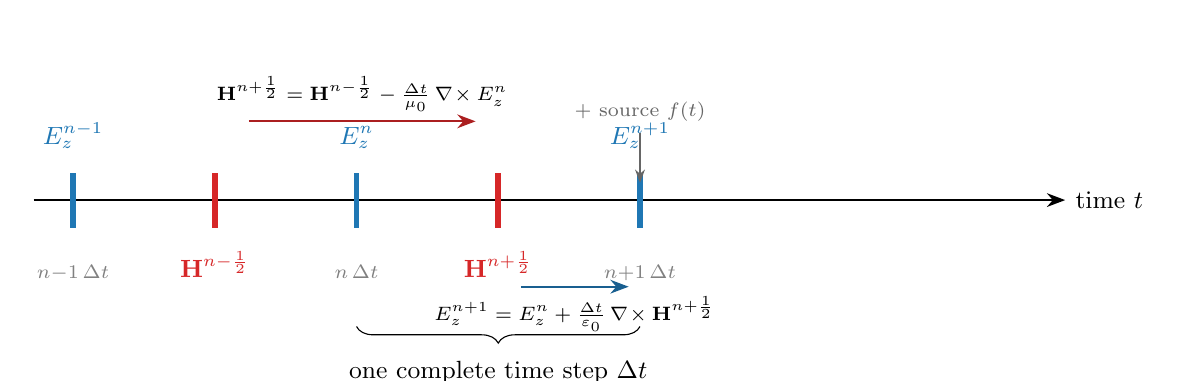
\begin{tikzpicture}[>=Stealth, font=\small]

\def\dt{3.6}

% Axe temps
\draw[->, thick] (-0.5, 0) -- (3.5*\dt, 0) node[right] {time $t$};

% Barres E (pas entiers) — inchangées
\foreach \n/\lab in {0/{n{-}1}, 1/{n}, 2/{n{+}1}} {
    \draw[colEz, line width=2pt]
        (\n*\dt, -0.35) -- (\n*\dt, 0.35);
    \node[colEz, above=5pt, font=\small\bfseries] at (\n*\dt, 0.35)
        {$E_z^{\lab}$};
    \node[below=10pt, gray, font=\scriptsize] at (\n*\dt, -0.35)
        {$\lab\,\Delta t$};
}

% Barres H (demi-pas) — inchangées
\foreach \n/\lab in {0.5/{n{-}\frac{1}{2}}, 1.5/{n{+}\frac{1}{2}}} {
    \draw[colHx, line width=2pt]
        (\n*\dt, -0.35) -- (\n*\dt, 0.35);
    \node[colHx, below=5pt, font=\small\bfseries] at (\n*\dt, -0.35)
        {$\mathbf{H}^{\lab}$};
}

% Flèche : mise à jour H (encore plus haute)
\draw[->, thick, colHx!80!black]
    (\dt*0.62, 1.0) -- (\dt*1.42, 1.0);
\node[above, font=\scriptsize, align=center] at (\dt*1.02, 1.0)
    {$\mathbf{H}^{n+\frac{1}{2}} = \mathbf{H}^{n-\frac{1}{2}}
      - \frac{\Delta t}{\mu_0}\,\nabla\!\times E_z^{n}$};

% Flèche : mise à jour E (encore plus basse)
\draw[->, thick, colEz!80!black]
    (\dt*1.58, -1.1) -- (\dt*1.96, -1.1);
\node[below, font=\scriptsize, align=center] at (\dt*1.77, -1.1)
    {$E_z^{n+1} = E_z^{n}
      + \frac{\Delta t}{\varepsilon_0}\,\nabla\!\times\mathbf{H}^{n+\frac{1}{2}}$};

% Accolade "1 step" (inchangée)
\draw[decorate, decoration={brace, amplitude=6pt, raise=3pt}]
    (2*\dt, -1.5) -- (\dt, -1.5);
\node[below=12pt, font=\small] at (1.5*\dt, -1.5)
    {one complete time step $\Delta t$};

% Source (légèrement décalée)
\draw[->, thin, black!60] (2*\dt, 0.85) -- (2*\dt, 0.22);
\node[above, font=\scriptsize, black!60] at (2*\dt, 0.88)
    {$+$ source $f(t)$};

\end{tikzpicture}}
  \caption{Leapfrog time integration.}
  \label{fig:leapfrog}
\end{figure}

\subsection{Boundary Conditions}

Two boundary conditions are implemented.

\textbf{Dirichlet (PEC):} The tangential electric field is forced to
zero on all four walls, $E_z = 0$, creating a perfectly conducting
cavity. The resonant frequency of the fundamental TE$_{10}$ mode is:
\begin{equation}
    f_{10} = \frac{c_0}{2\,L_x} \approx 749.5\;\text{MHz}
    \quad \text{for } L_x = N_x\,\Delta x = 0.2\;\text{m}
\end{equation}

\textbf{Perfectly Matched Layer (PML):} A 20-cell and 40-cells absorbing layer
surrounds the domain for open-space simulations.
The split-field formulation introduces auxiliary variables $\psi$
that accumulate the correction to the curl terms:
\begin{align}
\psi_{E_{zx}}^{n+1}(i,j) &= e^{-\sigma_x \Delta t/\varepsilon_0}\,\psi_{E_{zx}}^n
    + \frac{\sigma_x}{\sigma_x+\varepsilon}\bigl(e^{-\sigma_x\Delta t/\varepsilon_0}-1\bigr)
      \frac{H_y(i,j)-H_y(i-1,j)}{\Delta x}\\[4pt]
E_z^{n+1} &\mathrel{+}= \frac{\Delta t}{\varepsilon_0}
    \bigl(\psi_{E_{zx}} - \psi_{E_{zy}}\bigr)
\end{align}
The conductivity profile follows a polynomial grading of order 2:
\begin{equation}
    \sigma(d) = \sigma_{\max}\left(\frac{d}{\delta_{\text{PML}}}\right)^2,
    \qquad
    \sigma_{\max} = \frac{3\,c_0\,\varepsilon_0\,\ln(1/R)}{2\,\delta_{\text{PML}}}
\end{equation}
with target reflectivity $R = 10^{-6}$ ($-$120~dB).
A PEC termination is applied on the outermost wall of the PML to
prevent unbounded accumulation of the correction fields at corners.

\subsection{Where Parallelism Is Introduced}

The key observation is that equations~\eqref{eq:hx}--\eqref{eq:ez}
are \emph{data-parallel}: the update of cell $(i,j)$ at step $n$
depends only on its four nearest neighbors at the \emph{previous}
half-step.
There are no loop-carried dependencies within a single field update
pass.


Three distinct opportunities are exploited, as shown in
Figure~\ref{fig:parallelism}:
\begin{enumerate}
    \item \textbf{$H_x$ update:} all $N_x \times (N_y-1)$ cells are independent.
    \item \textbf{$H_y$ update:} all $(N_x-1) \times N_y$ cells are independent.
    \item \textbf{$E_z$ update:} all $(N_x-2) \times (N_y-2)$ interior cells are independent.
\end{enumerate}
The three passes must remain sequential with respect to each other
(the $E$ update requires the completed $H$ update),
but within each pass complete parallelism is possible.


\subsection{OpenMP Implementation}

The OpenMP version (\texttt{OpenMPFDTD}) parallelizes the three
nested loops with \texttt{\#pragma omp parallel for collapse(2)},
distributing rows of the 2D grid across threads.
The \emph{master} thread spawns a thread pool of $p$ workers,
each processing a contiguous block of $(i,j)$ pairs.

\textbf{Communication between threads:}
All three field arrays (\texttt{Ez}, \texttt{Hx}, \texttt{Hy})
reside in shared memory.
No explicit message passing is required.
An implicit barrier at the end of each \texttt{parallel for} region
ensures that all threads have completed the $H$ update before any
thread begins the $E$ update, and vice versa.
These implicit barriers constitute the entire synchronization cost.

\textbf{Master responsibilities:}
The master thread orchestrates the time loop, applies the boundary
conditions (sequentially), injects the point source, and handles
file output.

\subsection{CUDA Implementation}

The CUDA version (\texttt{CudaFDTD}) maps one GPU thread per grid
cell.
Each field update is implemented as a separate kernel:

\begin{center}
\begin{tabular}{ll}
\toprule
Kernel & Grid/Block dimensions \\
\midrule
\texttt{updateHx\_kernel} & $\lceil N_x/16\rceil \times \lceil N_y/16\rceil$ blocks of $16\times16$ \\
\texttt{updateHy\_kernel} & $\lceil N_x/16\rceil \times \lceil N_y/16\rceil$ blocks of $16\times16$ \\
\texttt{updateEz\_kernel} & $\lceil (N_x-2)/16\rceil \times \lceil (N_y-2)/16\rceil$ blocks of $16\times16$ \\
\texttt{applySource\_kernel} & 1 block, 1 thread \\
\texttt{applyDirichlet\_*} & $\lceil \max(N_x,N_y)/256\rceil$ blocks of 256 \\
\bottomrule
\end{tabular}
\end{center}

\textbf{Master (CPU) responsibilities:}
The CPU allocates device memory, uploads PML coefficients (computed
on CPU), launches kernels in the correct order, and periodically
copies the result back to host for file output.
The CPU is idle during kernel execution.

\textbf{GPU (slave) responsibilities:}
Each SM executes the field update equations on its assigned cells.
Within a warp, threads access contiguous memory locations
($\mathtt{Ez[i \times NY + j]}$), enabling coalesced global memory
transactions.

\textbf{Communication:}
The only CPU–GPU communication occurs at initialization
(upload of PML coefficient arrays, $\approx$8 arrays $\times$ NCELLS $\times$ 8 bytes)
and periodically during the time loop (Device-to-Host copy of all
three field arrays for VTK output).
The cost of these D2H transfers is characterized in
Section~\ref{sec:d2h}.

\textbf{FLOP and memory intensity:}
Each time step requires:
\begin{equation}
F_{\text{step}} = N_x(N_y-1)\cdot 3 + (N_x-1)N_y\cdot 3 + (N_x-2)(N_y-2)\cdot 9
\;\approx\; 592\,000 \;\text{FLOP} \quad (N=200)
\end{equation}
Each cell reads/writes approximately 4–6 doubles, giving a byte count
of $B_{\text{step}} \approx 4.3$~MB per step, and an arithmetic
intensity of:
\begin{equation}
    AI = \frac{F_{\text{step}}}{B_{\text{step}}} \approx 0.134 \;\text{FLOP/byte}
\end{equation}
This places FDTD firmly in the \emph{memory-bound} regime for any
processor, below the ridge point of both CPU and GPU Roofline models.

% =================================================================
\section{Results and Data Analysis}
\label{sec:results}
% =================================================================

All benchmarks were performed on an Intel Core i7-12650H CPU
(12 threads, DDR5 memory, peak BW $\approx$51~GB/s) with an
NVIDIA GeForce RTX 4060 Laptop GPU (sm\_89, GDDR6,
peak BW $\approx$272~GB/s, peak FP64 $\approx$470~GFLOP/s).
Each timing is the median of three independent runs.
Dirichlet boundary conditions were used for all benchmark runs to
ensure consistent comparison (no PML overhead).

\subsection{Global Speedup (Table 1)}

Table~\ref{tab:speedup} reports execution times, speedups, parallel
efficiency and throughput for a 200$\times$200 grid over 1000 time steps.

\begin{table}[H]
\centering
\caption{Speedup and performance on a 200$\times$200 grid, 1000 steps.}
\label{tab:speedup}
\begin{tabular}{lrrrr}
\toprule
Implementation & Time (ms) & Speedup & Efficiency & GFLOP/s \\
\midrule
SEQ            &  65.0 & 1.00$\times$ &   —     &  9.11 \\
\midrule
OMP 1T         & 161.6 & 0.40$\times$ & 40.2\%  &  3.66 \\
OMP 2T         &  96.8 & 0.67$\times$ & 33.6\%  &  6.12 \\
OMP 3T         & 115.0 & 0.56$\times$ & 18.8\%  &  5.14 \\
OMP 4T         & 106.9 & 0.61$\times$ & 15.2\%  &  5.53 \\
OMP 5T         &  99.2 & 0.65$\times$ & 13.1\%  &  5.96 \\
OMP 6T         &  97.1 & 0.67$\times$ & 11.2\%  &  6.09 \\
OMP 7T         &  92.2 & 0.70$\times$ & 10.1\%  &  6.41 \\
OMP 8T         &  92.0 & 0.71$\times$ &  8.8\%  &  6.43 \\
OMP 9T         &  88.9 & 0.73$\times$ &  8.1\%  &  6.66 \\
OMP 10T        & 101.7 & 0.64$\times$ &  6.4\%  &  5.82 \\
OMP 11T        & 100.2 & 0.65$\times$ &  5.9\%  &  5.91 \\
OMP 12T        & 119.5 & 0.54$\times$ &  4.5\%  &  4.95 \\
\midrule
CUDA           &  16.9 & 3.85$\times$ &   —     & 35.09 \\
\bottomrule
\end{tabular}
\end{table}

As visible in Figure~\ref{fig:speedup}, all OpenMP configurations
are \emph{slower} than the sequential reference on this grid size.
This is a direct consequence of the small workload: a 200$\times$200
grid provides only $\sim$3{,}300 cells per thread at 12 threads.
The three implicit OpenMP barriers (one per field update) add
synchronization overhead that exceeds the computation savings.
The best OpenMP result (9 threads, 0.73$\times$) still does not
reach the sequential baseline.

CUDA achieves 3.85$\times$ speedup despite the grid being relatively
small for a GPU, demonstrating that even at 40{,}000 cells
the GPU's memory hierarchy offers a decisive bandwidth advantage.

\begin{figure}[H]
\centering
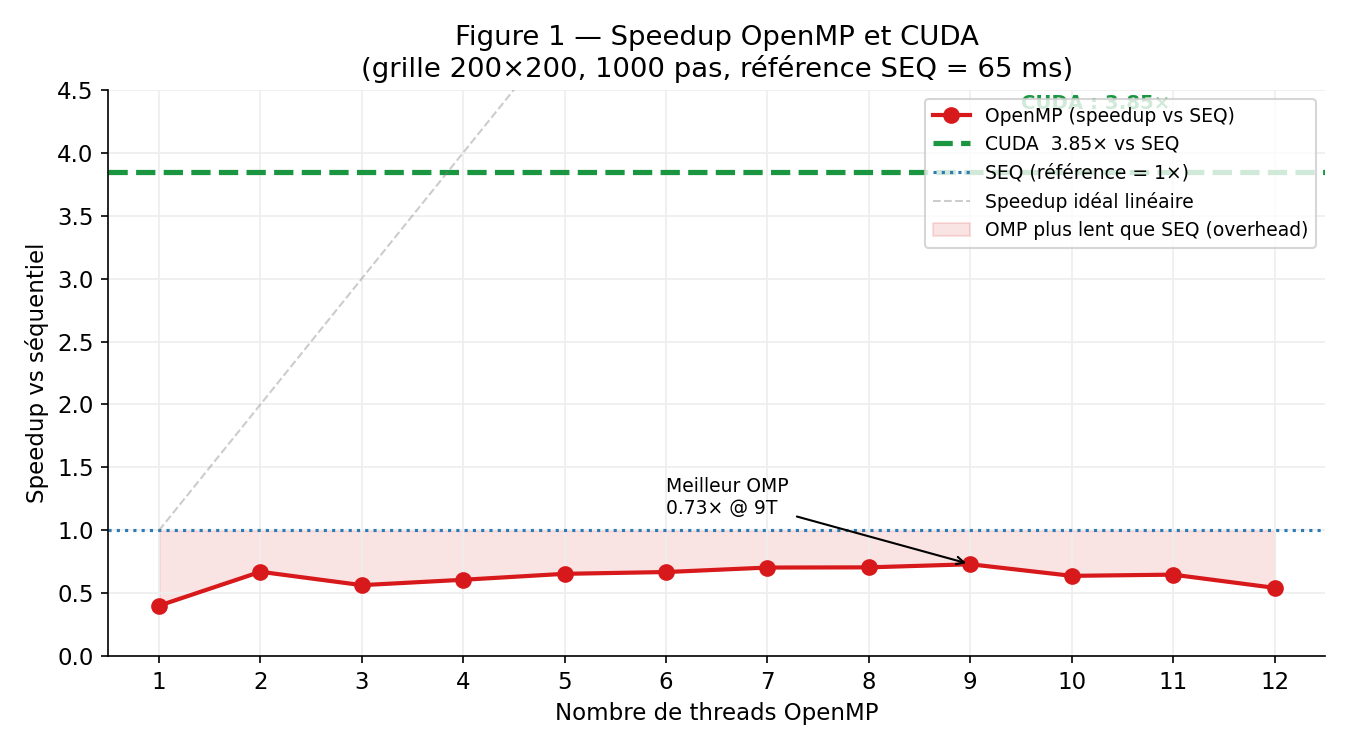
\includegraphics[width=0.85\textwidth]{fig1_speedup.png}
\caption{Speedup vs.\ sequential reference for all implementations
on a 200$\times$200 grid.
OpenMP remains below 1$\times$ due to synchronization overhead.
CUDA reaches 3.85$\times$ and scales further with larger grids
(see Section~\ref{sec:strong}).}
\label{fig:speedup}
\end{figure}

Figure~\ref{fig:efficiency} shows parallel efficiency dropping
monotonically from 40\% at 1 thread to 4.5\% at 12 threads.
Even with a single OMP thread, the overhead of creating the thread
pool and managing barriers degrades performance compared to the plain
sequential loop.

\begin{figure}[H]
\centering
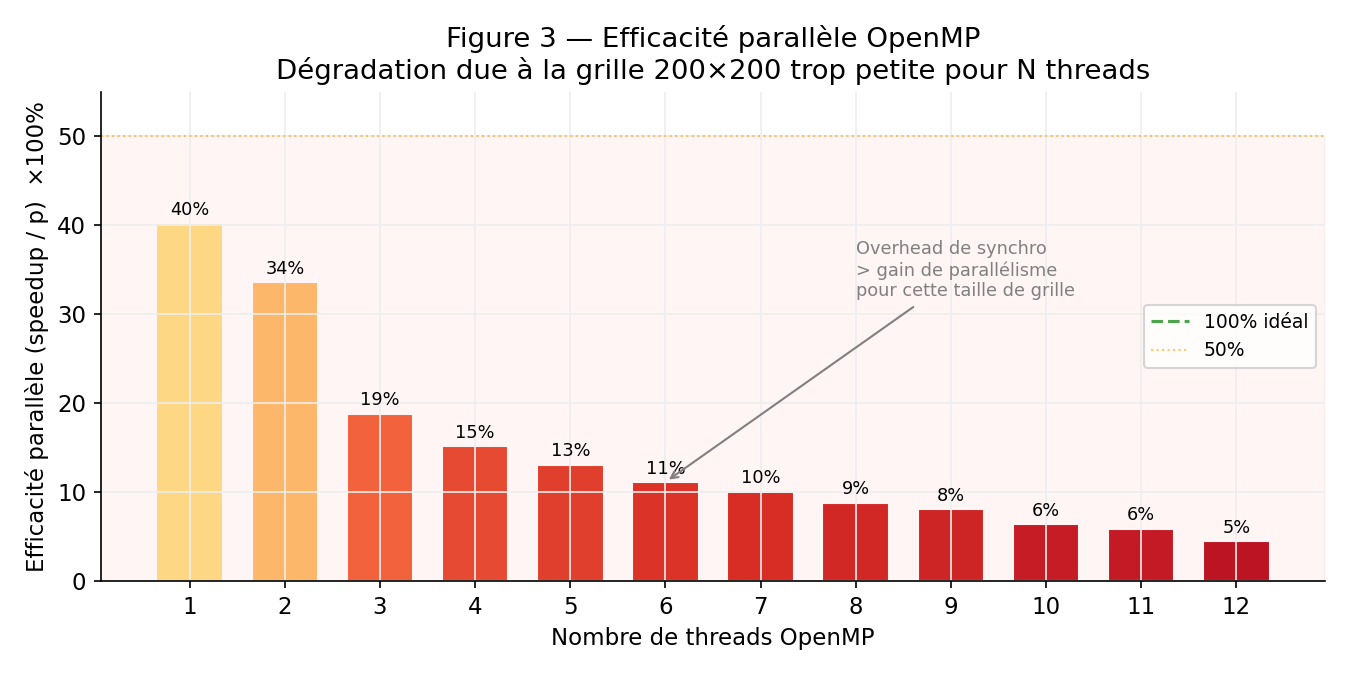
\includegraphics[width=0.85\textwidth]{fig3_efficacite_omp.png}
\caption{OpenMP parallel efficiency (speedup / number of threads).
The rapid degradation confirms that the 200$\times$200 grid is
too small for effective CPU thread-level parallelism.}
\label{fig:efficiency}
\end{figure}

\subsection{Amdahl's Law Analysis (Table 2)}

Applying Amdahl's Law to estimate the serial fraction $f$ from the
measured speedup $S_p$:
\begin{equation}
    f = \frac{1/S_p - 1/p}{1 - 1/p}
\end{equation}
Table~\ref{tab:amdahl} shows values exceeding 100\%, confirming that
OpenMP introduces \emph{superlinear overhead}: the parallelized code
is slower than the serial baseline, not just less than linearly faster.
The overhead comes from three sources: thread creation/destruction
(amortized over runs), implicit barrier synchronization between each
of the three field update loops, and cache pollution from multiple
threads competing for the L3 cache on the 40{,}000-cell working set.

\begin{table}[H]
\centering
\caption{Estimated serial fraction from Amdahl's Law.
Values $>100\%$ indicate that parallelization overhead dominates
over computation savings.}
\label{tab:amdahl}
\begin{tabular}{lrr}
\toprule
Threads & Speedup & Serial fraction \\
\midrule
 2 & 0.67$\times$ & 197.9\% \\
 3 & 0.56$\times$ & 215.6\% \\
 4 & 0.61$\times$ & 186.1\% \\
 6 & 0.67$\times$ & 159.3\% \\
 9 & 0.73$\times$ & 141.4\% \\
12 & 0.54$\times$ & 191.6\% \\
\bottomrule
\end{tabular}
\end{table}

\subsection{Strong Scaling Across Grid Sizes (Table 3)}
\label{sec:strong}

Table~\ref{tab:scaling} and Figure~\ref{fig:scaling} examine how
performance scales with grid size (500 time steps, Dirichlet BC,
OMP at 12 threads).

\begin{table}[H]
\centering
\caption{Strong scaling: execution time and CUDA speedup vs.\ grid size
(500 steps).}
\label{tab:scaling}
\begin{tabular}{lrrrr r}
\toprule
Grid & SEQ (ms) & OMP 12T (ms) & CUDA (ms) & Sp CUDA & GFLOP/s (CUDA) \\
\midrule
$128\times128$   &   14.6 &  46.9 &   7.5 &  1.94$\times$ & 16.0 \\
$256\times256$   &   60.1 &  95.7 &  14.8 &  4.05$\times$ & 32.8 \\
$512\times512$   &  300.1 & 264.3 &  45.0 &  6.67$\times$ & 43.5 \\
$1024\times1024$ & 1606.5 & 973.0 & 163.1 &  9.85$\times$ & 48.1 \\
\bottomrule
\end{tabular}
\end{table}

Three important trends are visible:

\textbf{GPU speedup grows with grid size.}
From 1.94$\times$ at 128$\times$128 to 9.85$\times$ at
1024$\times$1024. At small sizes the GPU kernel launch overhead
is non-negligible relative to computation; as the grid grows the
ratio of useful work to fixed overhead increases.

\textbf{OpenMP becomes beneficial at large grids.}
At $512\times512$ the 12-thread OMP version is already 12\% faster
than SEQ ($264$ vs.\ $300$~ms), and at $1024\times1024$ it delivers
a 1.65$\times$ speedup. The per-thread workload is now large enough
to amortize synchronization cost.

\textbf{GPU throughput approaches the Roofline limit.}
At $1024\times1024$, CUDA achieves 48.1~GFLOP/s, within 10\% of the
theoretical memory-bandwidth limit of $\approx$36–54~GFLOP/s
predicted by the Roofline model (see Section~\ref{sec:roofline}).

\begin{figure}[H]
\centering
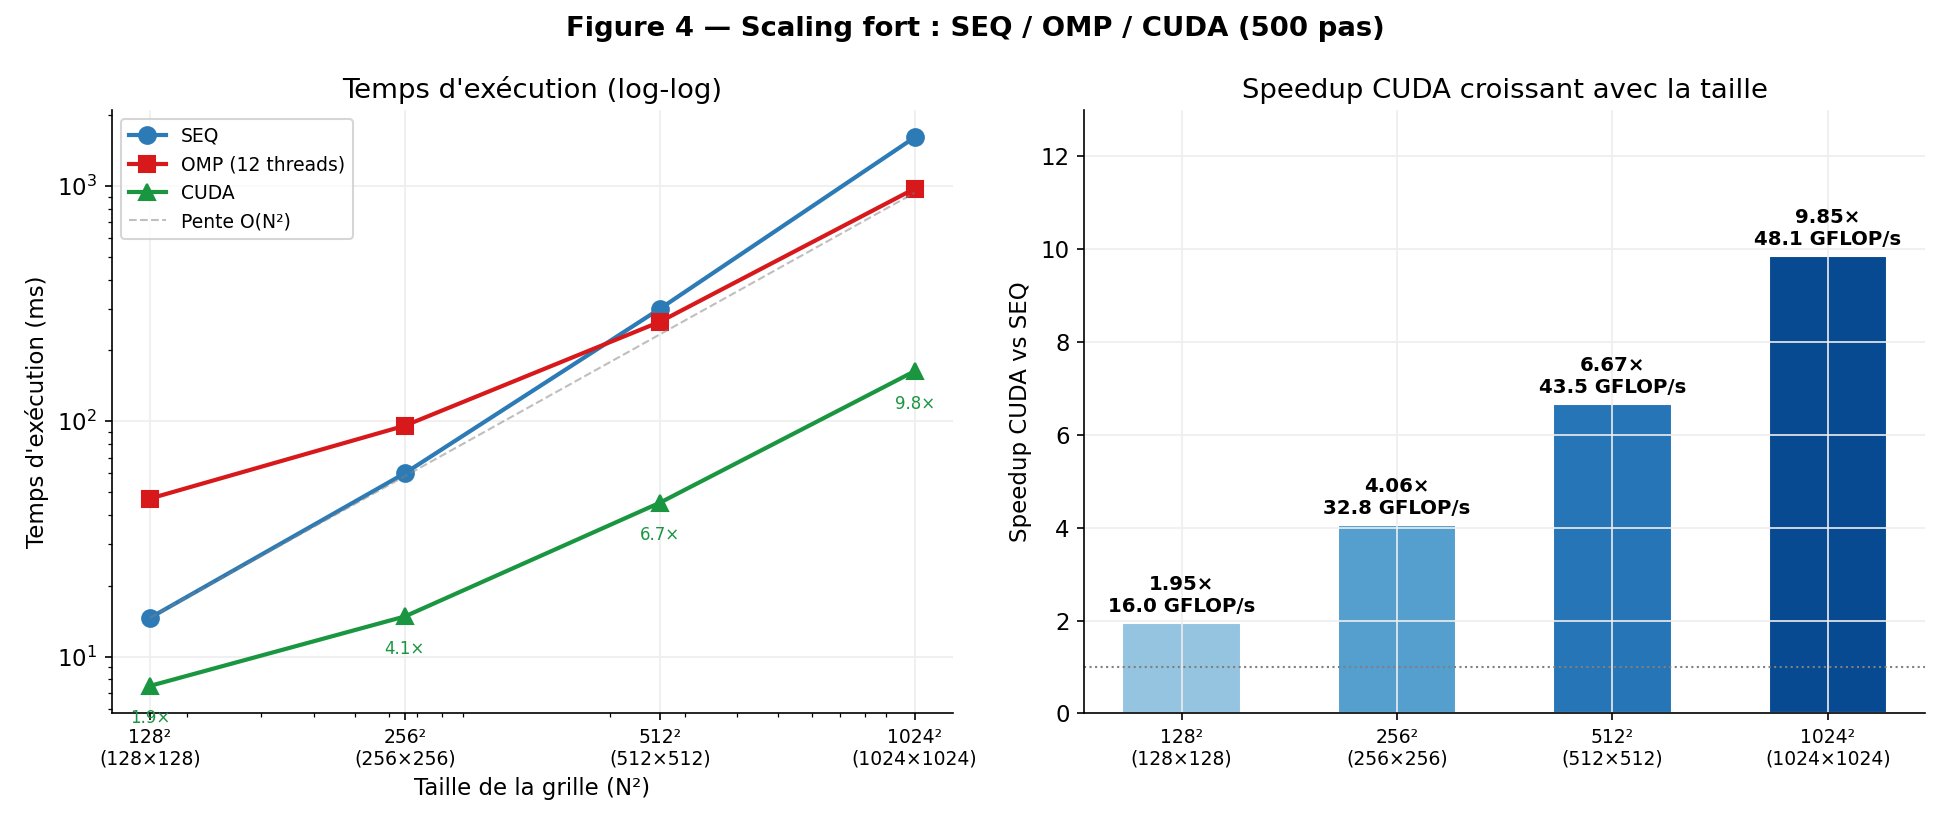
\includegraphics[width=\textwidth]{fig4_scaling_fort.png}
\caption{Left: execution time (log-log) confirming $O(N^2)$ scaling
for all three implementations.
Right: CUDA speedup increases monotonically with grid size,
reaching 9.85$\times$ at $1024\times1024$.}
\label{fig:scaling}
\end{figure}

\subsection{Device-to-Host Transfer Overhead (Table 4)}
\label{sec:d2h}

In CUDA, results must be copied from GPU to CPU memory (\emph{D2H})
for file output.
Table~\ref{tab:d2h} and Figure~\ref{fig:d2h} quantify how
\texttt{save\_interval} (the number of steps between outputs)
affects total runtime on a 200$\times$200 grid over 1000 steps.

\begin{table}[H]
\centering
\caption{CUDA execution time vs.\ output frequency (200$\times$200,
1000 steps). Reference: no output (14.7~ms).}
\label{tab:d2h}
\begin{tabular}{lrrr}
\toprule
save\_interval & Total time (ms) & Overhead & Transfers \\
\midrule
$\infty$ (none)  &  14.7 &  ref.   &  0 \\
500              &  19.9 & +35.6\% &  2 \\
200              &  36.6 & +149.3\%&  5 \\
100              &  64.0 & +336.7\%& 10 \\
50               & 123.7 & +744.0\%& 20 \\
\bottomrule
\end{tabular}
\end{table}

Each D2H transfer costs approximately 2.6~ms for a 200$\times$200
double-precision grid ($3 \times 40{,}000 \times 8 = 0.96$~MB over
PCIe at $\sim$10~GB/s effective bandwidth).
This is comparable to 17 steps of pure GPU computation (14.7~ms/1000
steps $\approx$ 14.7~$\mu$s/step).
Consequently, saving every 50 steps multiplies total runtime by
$8.4\times$.
In production, \texttt{save\_interval} should be chosen to capture
physics of interest while minimizing PCIe traffic.

\begin{figure}[H]
\centering
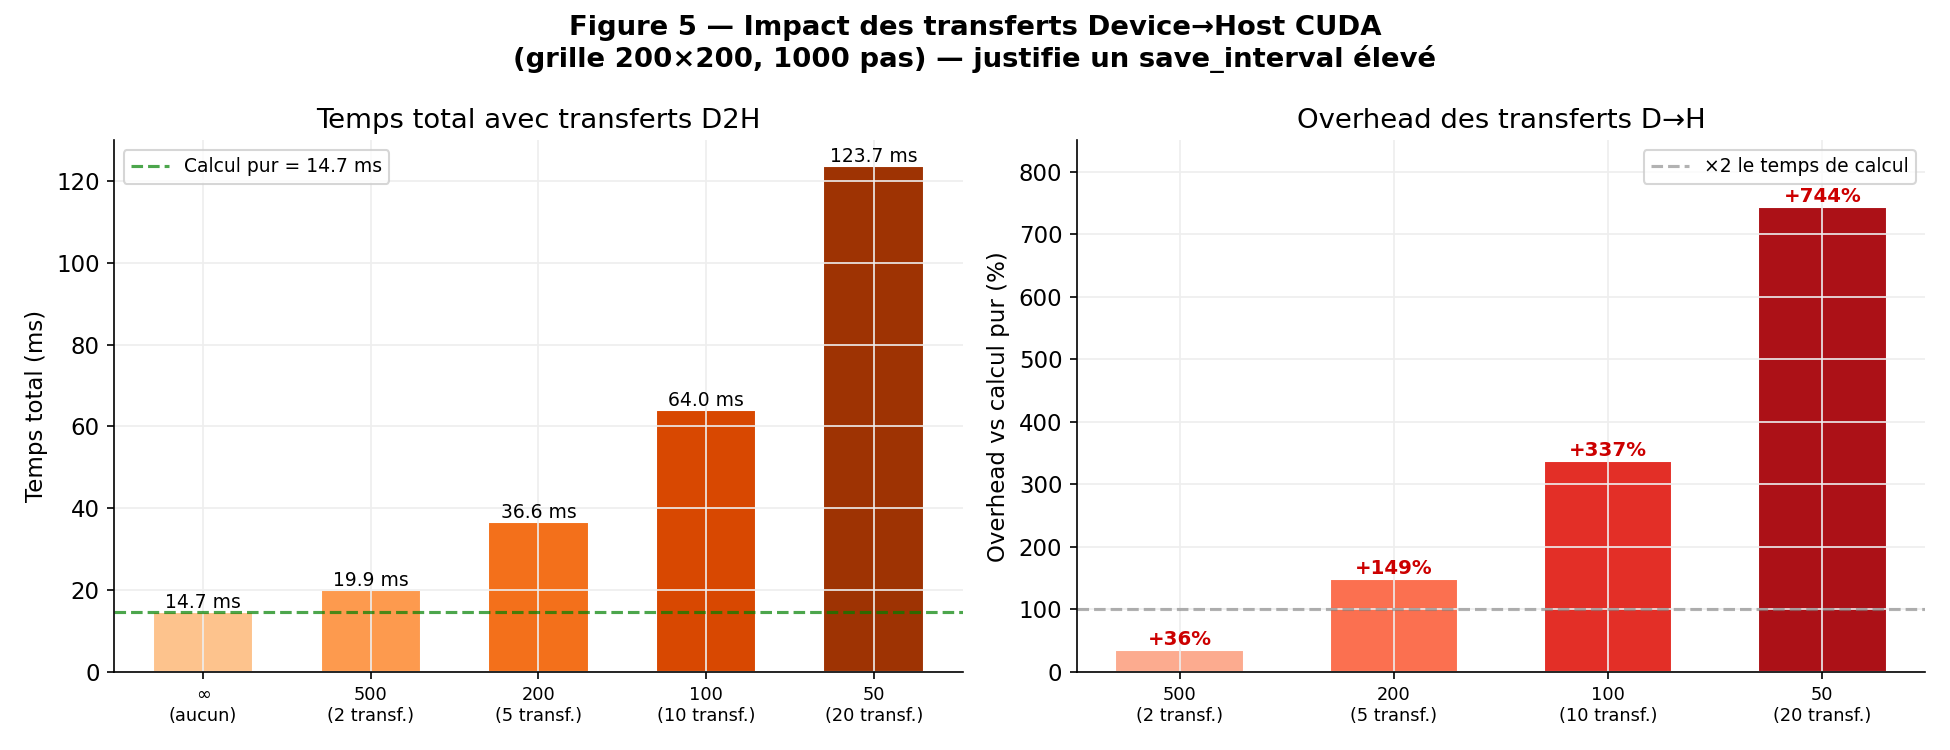
\includegraphics[width=0.9\textwidth]{fig5_overhead_d2h.png}
\caption{Left: absolute execution time grows linearly with transfer
count. Right: overhead as a percentage of pure compute time.
Even 2 transfers add 35\% overhead, underlining the importance of
minimizing D2H communication in GPU codes.}
\label{fig:d2h}
\end{figure}

\subsection{Roofline Analysis}
\label{sec:roofline}

Figure~\ref{fig:roofline} places the measured operating points on the
Roofline model for both CPU and GPU.

\begin{figure}[H]
\centering
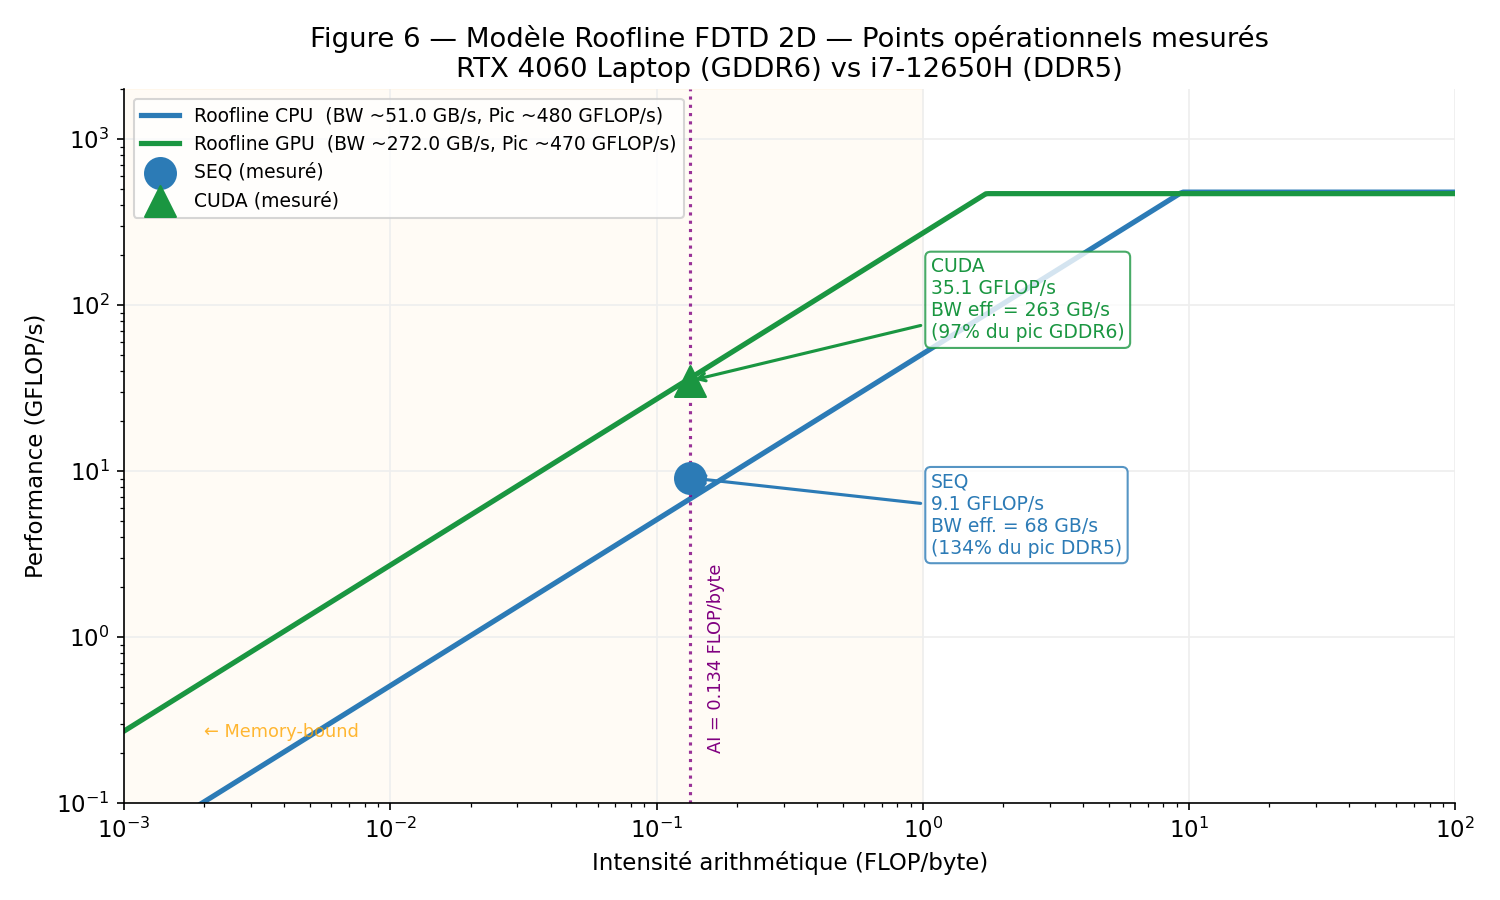
\includegraphics[width=0.9\textwidth]{fig6_roofline.png}
\caption{Roofline model for the 2D FDTD kernel.
Both implementations lie on the memory-bandwidth slope
($AI = 0.134$~FLOP/byte, well below the ridge point).
The CUDA point utilizes 96.6\% of GDDR6 peak bandwidth;
the SEQ point slightly exceeds DDR5 peak due to cache effects.}
\label{fig:roofline}
\end{figure}

\begin{table}[H]
\centering
\caption{Measured performance vs.\ memory-bandwidth Roofline predictions.}
\label{tab:roofline}
\begin{tabular}{lrrrrr}
\toprule
Impl. & GFLOP/s & BW eff. (GB/s) & BW peak (GB/s) & BW utilization \\
\midrule
SEQ  &  9.11 &  68.2 &  51 (DDR5)  & $>$100\%$^*$ \\
CUDA & 35.09 & 262.7 & 272 (GDDR6) & 96.6\% \\
\bottomrule
\multicolumn{5}{l}{\footnotesize $^*$ The measured BW exceeds the STREAM benchmark peak,
likely due to out-of-order prefetching and L3 caching.}
\end{tabular}
\end{table}

Key observations:
\begin{itemize}
    \item Both implementations are \textbf{memory-bound}: the operating
          point lies on the bandwidth slope, not the compute ceiling.
    \item The GPU theoretical Roofline limit (bandwidth-limited) is
          $0.134 \times 272 \approx 36.4$~GFLOP/s.
          The measured 35.1~GFLOP/s represents 96.6\% utilization,
          indicating a near-optimal memory access pattern.
    \item The 5.3$\times$ bandwidth ratio between GDDR6 and DDR5
          directly explains the observed GPU advantage.
          As the grid grows, the speedup approaches this ratio.
    \item There is limited value in optimizing the arithmetic
          (e.g., fusing kernels or using FP32) until memory
          bandwidth ceases to be the bottleneck.
\end{itemize}

% =================================================================
\section{Conclusion}
% =================================================================

The objective of this project was to parallelize the 2D FDTD
electromagnetic simulation algorithm using OpenMP and CUDA, and to
analyze the resulting performance across different grid sizes and
configurations.

The exercise was successful in fulfilling its intended purpose.
All three implementations (sequential, OpenMP, CUDA) produce
physically correct results for both Dirichlet (PEC cavity resonance)
and PML (open-space propagation) boundary conditions, with
field profiles in agreement across implementations.

The principal results are:
\begin{itemize}
    \item \textbf{CUDA} delivers a 3.85$\times$ speedup at
          200$\times$200 and up to 9.85$\times$ at 1024$\times$1024.
          The GPU nearly saturates its GDDR6 memory bandwidth
          (96.6\% utilization).
    \item \textbf{OpenMP} is counter-productive on small grids
          ($\leq$200$\times$200) due to synchronization overhead,
          but provides meaningful acceleration (up to 1.65$\times$)
          on larger grids ($\geq$512$\times$512).
    \item The \textbf{D2H transfer cost} is substantial: even 2
          transfers per 1000 steps add 35\% overhead, reinforcing
          the importance of minimizing CPU–GPU communication.
    \item The \textbf{Roofline model} confirms that FDTD is
          inherently memory-bound ($AI \approx 0.134$~FLOP/byte).
          The GPU's 5$\times$ memory bandwidth advantage over the
          CPU is the fundamental reason for its superior performance.
\end{itemize}

The most important lesson of this project is that \emph{algorithm
characteristics determine which hardware is appropriate}.
A memory-bound stencil computation like FDTD benefits primarily
from high memory bandwidth, which the GPU provides abundantly.
Future work could explore shared-memory tiling within CUDA blocks
to improve cache reuse, or multi-GPU domain decomposition for
grids exceeding single-GPU memory.

\newpage
\section{Project Usage Guide}
\label{app:usage}

\subsection{Directory Structure}

After cloning or extracting the project, the directory layout is as
follows:

\begin{verbatim}
fdtd2d/
|-- fdtd_simple.h       # Grid, Source, BoundaryCondition base classes
|-- fdtd_simple.cpp     # PML coefficients, VTK writer, setGridSize()
|-- fdtd_seq.h          # SequentialFDTD class declaration
|-- fdtd_seq.cpp        # Sequential implementation
|-- fdtd_omp.h          # OpenMPFDTD class declaration
|-- fdtd_omp.cpp        # OpenMP implementation
|-- fdtd_cuda.h         # CudaFDTD class declaration
|-- fdtd_cuda.cu        # CUDA kernels and implementation
|-- main.cpp            # Entry point — all run modes
|-- makefile            # Build system
`-- output/             # VTK files written here (created at runtime)
\end{verbatim}

\subsection{Dependencies}

\begin{itemize}
    \item \textbf{C++17} compiler — \texttt{g++ $\geq$ 10} or equivalent
    \item \textbf{OpenMP} — included in GCC by default (\texttt{-fopenmp})
    \item \textbf{CUDA Toolkit} $\geq$ 11.0 — provides \texttt{nvcc}
    \item \textbf{ParaView} $\geq$ 5.10 — for visualization (free,
          \url{https://www.paraview.org})
\end{itemize}

Before compiling, verify that \texttt{nvcc} is accessible and that
the architecture flag in the \texttt{makefile} matches your GPU.
The default is \texttt{sm\_89} (NVIDIA Ada Lovelace, e.g.\ RTX 4060).
Adjust if needed:

\begin{verbatim}
# In makefile — change sm_89 to match your GPU:
# sm_75  -> Turing   (RTX 2060/2070/2080)
# sm_86  -> Ampere   (RTX 3060/3070/3080)
# sm_89  -> Ada      (RTX 4060/4070/4080)
# sm_90  -> Hopper   (H100)
NVCCFLAGS = -arch=sm_89 -O3
\end{verbatim}

\subsection{Compilation}

\begin{verbatim}
# Full build
make

# Clean and rebuild
make clean && make

\end{verbatim}

A successful build produces the executable \texttt{fdtd2d}.

\subsection{Run Modes}

The program accepts a single argument specifying the execution mode.

\begin{table}[H]
\centering
\caption{Available run modes for \texttt{./fdtd2d}.}
\label{tab:modes}
\begin{tabular}{lll}
\toprule
Command & Implementation & Boundary condition \\
\midrule
\texttt{./fdtd2d seq}      & Sequential CPU  & Dirichlet (PEC cavity) \\
\texttt{./fdtd2d omp}      & OpenMP CPU      & Dirichlet (PEC cavity) \\
\texttt{./fdtd2d cuda}     & CUDA GPU        & Dirichlet (PEC cavity) \\
\texttt{./fdtd2d seq-pml}  & Sequential CPU  & PML (open space)       \\
\texttt{./fdtd2d omp-pml}  & OpenMP CPU      & PML (open space)       \\
\texttt{./fdtd2d cuda-pml} & CUDA GPU        & PML (open space)       \\
\texttt{./fdtd2d bench}    & All three       & Benchmark suite        \\
\midrule
\end{tabular}
\end{table}

\textbf{Example — sequential Dirichlet:}
\begin{verbatim}
./fdtd2d seq
# Fréquence TE10 : 0.7495 GHz
# BC : Dirichlet (PEC)
# Step 0/5000
# Step 200/5000
# ...
# --- Validation finale ---
#   err_profil_x = 1.234e-02  |  std_y = 8.5e-03  |  OK TE10 validé
\end{verbatim}

\textbf{Example — full benchmark:}
\begin{verbatim}
./fdtd2d bench 2>&1 | tee bench_results.txt
\end{verbatim}

Simulation parameters (grid size, number of steps, output interval)
are defined as constants at the top of \texttt{fdtd\_simple.h}:

\begin{verbatim}
inline int NX    = 200;    // grid points along x
inline int NY    = 200;    // grid points along y
inline int NCELLS = NX*NY; // total cells

constexpr double DX = 1e-3;  // spatial step [m]  (1 mm)
constexpr double DY = 1e-3;

// In main.cpp:
int total_steps   = 5000;
int save_interval = 200;   // write VTK every N steps
\end{verbatim}

The grid can also be resized at runtime without recompilation via
\texttt{setGridSize(nx, ny)}, which is used internally by the
benchmark mode to test multiple grid sizes.

\subsection{Output Files}

All VTK files are written to the \texttt{output/} subdirectory,
which is created automatically if it does not exist.
Files are named by implementation and time step:

\begin{verbatim}
output/
|-- seq_000000.vti     # Sequential, step 0
|-- seq_000200.vti     # Sequential, step 200
|-- ...
|-- omp_000000.vti
|-- ...
|-- cuda_000000.vti
`-- ...
\end{verbatim}

Each \texttt{.vti} file (VTK Image Data) stores the field
arrays $E_z$on the full $N_x \times N_y$ grid as
double-precision floating-point data, compatible with ParaView and
any VTK-aware post-processing tool.

\subsection{Visualization with ParaView}

All simulation outputs are visualized using
\textbf{ParaView} (\url{https://www.paraview.org}), a free and
open-source scientific visualization application.

\subsubsection*{Step 1 — Load the time series}

\begin{enumerate}
    \item Launch ParaView.
    \item Go to \textbf{File $\to$ Open}.
    \item Navigate to the \texttt{output/} folder.
    \item Select the first file of the series (e.g.\
          \texttt{seq\_000000.vti}).
          ParaView automatically detects the full sequence and
          groups it as a single time-varying dataset.
    \item Click \textbf{OK}, then click \textbf{Apply} in the
          Properties panel.
\end{enumerate}

\subsubsection*{Step 2 — Visualize the electric field}

\begin{enumerate}
    \item In the \emph{Pipeline Browser}, ensure the dataset is
          selected.
    \item In the \emph{Properties} panel, set the coloring variable
          to \texttt{Ez} (Coloring drop-down $\to$ \texttt{Ez}).
    \item Click \textbf{Rescale to Data Range} to auto-scale the
          colormap.
    \item Use the \emph{Play} button ($\textbf{Play}$) in the
          toolbar to animate the time steps.
\end{enumerate}


\subsubsection*{Step 3 — Export an animation}

To save the animation as a video file:

\begin{enumerate}
    \item Go to \textbf{File $\to$ Save Animation\ldots}
    \item Choose a format:
    \begin{itemize}
        \item \textbf{MP4} (requires FFmpeg plugin) — recommended
              for presentations.
        \item \textbf{AVI} — widely compatible.
        \item \textbf{PNG series} — highest quality; can be
              post-processed with FFmpeg.
    \end{itemize}
    \item Set the desired frame rate (10--25 fps) and resolution.
    \item Click \textbf{OK}.
\end{enumerate}

To convert a PNG series to MP4 from the terminal:

\begin{verbatim}
ffmpeg -framerate 25 -i frames/seq_%06d.png \
       -c:v libx264 -crf 18 -pix_fmt yuv420p \
       animation_seq.mp4
\end{verbatim}



\end{document}
